\documentclass{article}
\usepackage[utf8]{inputenc}
\usepackage[spanish]{babel}
\usepackage{listings}
\usepackage{graphicx}
\graphicspath{ {images/} }
\usepackage{cite}

\begin{document}

\begin{titlepage}
    \begin{center}
        \vspace*{1cm}
            
        \Huge
        \textbf{Memorias de un computador}
            
        \vspace{0.5cm}
        \LARGE
        Memorias, función, formas de trabajo y tipos
            
        \vspace{1.5cm}
            
        \textbf{Cristiam Gutierrez Jiménez}
            
        \vfill
            
        \vspace{0.8cm}
            
        \Large
        Facultad de Ingeniería de Telecomunicaciones\\
        Universidad de Antioquia\\
        Medellín\\
        Septiembre de 2020
            
    \end{center}
\end{titlepage}

\tableofcontents

\section{Memoria de un computador}

La memoria de una computadora es el dispositivo/s donde se almacena información de forma temporal o permanente, y de manera lógica por medio del sistema binario de unos y ceros, determinar si los datos son grabados de manera temporal o permanente depende de la clasificación de la memoria que se esté usando.\cite{NormaIPC}\\

En nuestro computador contamos con muchos tipos de memoria y los mencionaremos a medida que avancemos en el texto, pero podemos mencionar que las memorias son:

\section{Tipos de memoria}



\subsection{Memoria RAM}
Es la cual nos permite la lectura escritura e instrucciones, pero es volátil, lo cual profundizaremos más adelante, y a su vez se subdividen en.

\begin{itemize}
    \item Estáticas
    \item Dinámicas
\end{itemize}

la memoria de acceso aleatorio RAM por sus siglas en inglés es de Gran importancia en la computadora, ya que de esto depende qué tanta información se pueda procesar al ejecutar un programa, entre mayor sea el tamaño de la RAM mayor es la capacidad de trabajo de la computadora.\\


\begin{figure}[h]
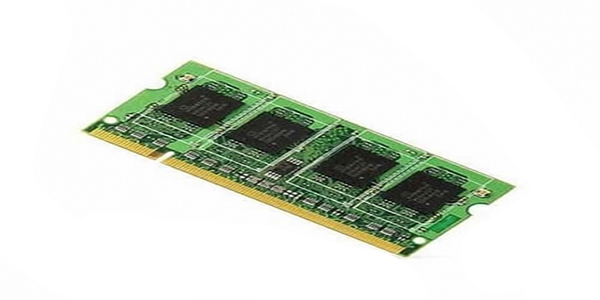
\includegraphics[width=4cm]{Memoria-ram.png}
\centering
\caption{Memoria RAM}
\label{fig:Memoria-ram}
\end{figure}


La RAM se encuentra constituida en módulos y se compone de circuitos integrados soldados sobre un circuito impreso independiente con pines o conectores para colocarlos en unas ranuras especiales dentro de la Tarjeta Madre o Main Board.\\

Normalmente se pueden colocar de 2 a 4 módulos por tarjeta madre. la unidad de memoria son los bytes y se utilizan los prefijos mega 1000000 o giga mil millones para cuestiones prácticas, los módulos de memoria comercialmente más pequeños son de 512 megabytes y los más grandes de 16 gigabytes. Aunque continúa el desarrollo de capacidades mayores.\\

\subsubsection{Estructura interna de la RAM dinámica DRAM}
La DRAM es una RAM que se encuentra constituida internamente por un circuito integrado hecho de millones de capacitores y transistores, para el caso de las RAM dinámicas que son las de uso más común en la actualidad los transistores y capacitores están colocados en pares para formar una celda de memoria en la que si el capacitor se encuentra cargado se considera un 1 lógico, y si el capacitor se encuentra descargado se considera un 0 lógico.\\

El transistor de la RAM funciona como un switch que permite que la circuitería de control del chip de memoria pueda leer o cambiar el dato de la celda de memoria, Las DRAM Ram dinámicas necesitan que los capacitores constantemente sean recargados ya que de otra manera se descargarán y perderán la información almacenada, para este proceso el controlador de memoria o el CPU necesitan leer la memoria y volver a escribir en ella millones de veces por segundo.\\

\subsubsection{Funcionamiento de la DRAM o RAM dinámica:}

\begin{figure}[h]
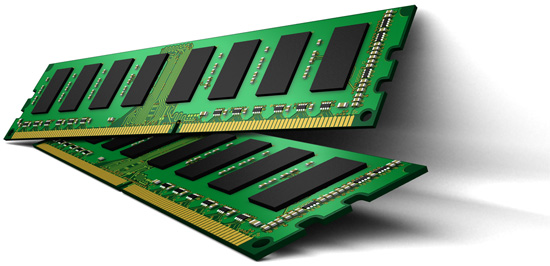
\includegraphics[width=4cm]{DRAM.png}
\centering
\caption{Memoria DRAM}
\label{fig:Memoria DRAM}
\end{figure}


La RAM está conformada de una rejilla bidimensional de bits, la configuración de las celdas de memoria es un arreglo de columnas llamadas líneas de bits y un arreglo de renglones llamados líneas de palabras, a la intersección de estos dos elementos se le llama dirección de la celda de memoria 1 DRAM; funciona mandando una carga al selector de dirección de columna para activar el transistor en cada bit de la columna cuando se requiere escribir los renglones que contendrán el estado nuevo que el capacitor tendrá, y en el caso de la lectura un amplificador de detección determinará el nivel de carga en el capacitor, si es más del 50 por ciento se considerará un 1 lógico, de lo contrario se tomará como un 0 lógico.

\subsubsection{Funcionamiento de la RAM estática SRAM:}

\begin{figure}[h]
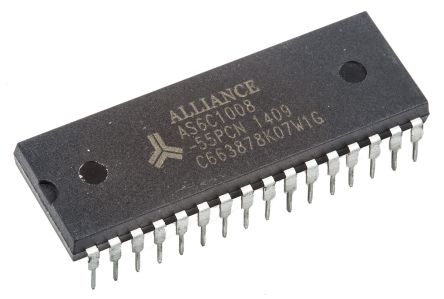
\includegraphics[width=4cm]{SRAM.png}
\centering
\caption{Memoria SRAM}
\label{fig:Memoria SRAM}
\end{figure}


En el caso de las memorias estáticas SRAM el funcionamiento es distinto, ya que éstas se encuentran integradas por flip-flops los cuales forman una celda de memoria, estos componentes lógicos requieren de mayor número de transistores lo que hace que la memoria ocupe mayor espacio disminuyendo su capacidad de almacenamiento por chip, la ventaja que ofrece esta memoria sobre la de SRAM es que no requiere de una reescritura constante lo que la hace mucho más rápida, sin embargo es más costosa y Normalmente se utiliza como memoria caché del microprocesador, los módulos de memoria se encuentran construidos en arreglos de varios chips dependiendo de la capacidad de estos, normalmente expresados en megabytes se obtiene la capacidad total del módulo es decir si se encuentra un módulo con la leyenda 4 * 32, se tienen cuatro chips con capacidad de 32 megabytes cada uno, es decir que su capacidad es de 128 megabytes. Y si consideramos que un byte contiene 8 bits su capacidad total es de 16 megabytes.

\subsubsection{Estructura lógica de una memoria RAM:}
la estructura lógica o asignación de zonas de una memoria RAM es la siguiente;

\begin{itemize}
    \item Memoria base: es la zona donde se almacena la mayoría de los programas que el usuario utiliza.
    \item Memoria Superior y reservada: carga unas estructuras llamadas páginas de intercambio de información con espacios asignados para el sistema dentro de la memoria superior, normalmente para la carga de drivers.
    \item Memoria Expandida: en ella se almacenan todas las aplicaciones que requieren mayor memoria y no caben en la memoria base, la memoria RAM se comunica con el puente Norte para proporcionar información al microprocesador o almacenar datos que pueden provenir del mismo microprocesador de periféricos o del disco duro.
\end{itemize}

\subsection{Los discos duros (HHDD)}

Los discos duros que son el cuarto de gran archivo del que hablamos antes, son uno de los dispositivos que más tiempo hace que no evolucionan y son el gran cuello de botella del PC, son sin duda el dispositivo más lento de todo el computador, y el que hace que tenga que esperar que los programas carguen en muchos casos.\\


\begin{figure}[h]
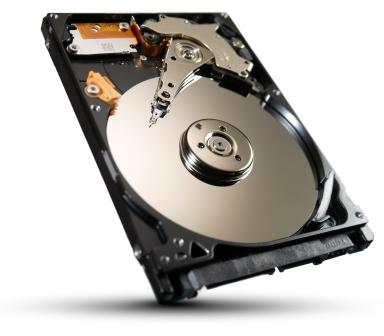
\includegraphics[width=4cm]{HHDD.png}
\centering
\caption{Disco duro HHDD}
\label{fig:Disco duro HHDD}
\end{figure}


Cuando quieres abrir un programa se manda la orden para que una serie de datos se carguen en la RAM esto sería el equivalente a mover todo lo que necesitas para trabajar ese día del archivo a la estantería, un disco duro tiene una aguja magnética que lee trazos dentro de un disco de acero magnetizado, es un poco como un tocadiscos para dar una idea. En realidad, tiene varios discos dentro, cada vez que se solicitan datos al disco duro tiene que buscarlo dentro de estos discos, el disco tiene una tabla donde tiene apuntado el sitio de cada uno de esos archivos, esto se llama el sistema de ficheros, lo que es el equivalente a tener un pequeño índice para saber en qué estantería se encuentra cada uno de los informes que necesitamos de nuestro cuarto de gran archivo.\\ 

Cuando al disco se le pide un archivo, se mira la tabla del sistema de ficheros y luego se va a buscar los datos a la posición especificada entonces viene la pregunta…\\

\subsubsection{¿en qué momento se ralentiza tu PC por el disco duro?}

Pues esto ocurre cuando tienes que ir a buscar o guardar informes al gran archivo es decir cada vez que se leen datos o se escriben datos a disco, el ejemplo más claro es copiar un archivo o cuando Windows arranca, lo que hace es cargar un montón de datos en la RAM para poder trabajar, Lo mismo ocurre cuando cargas un programa o durante la pantalla de carga de un videojuego.\\ 

Ese es el momento en el que realmente necesitas traerte los archivos del cuarto de gran archivo y ponerlos en la estantería, Ahora, ¿qué pasa cuando tu estantería es demasiado pequeña para todo lo que tienes que guardar? Pues que no cabe, y la solución que tiene el PC para solucionar este tipo de situaciones es utilizar como RAM parte del disco duro, cuando el PC se ve obligado a usar este método como podrás imaginar todo se pone lento en realidad.

\subsection{SSD discos de estado solido}

\begin{figure}[h]
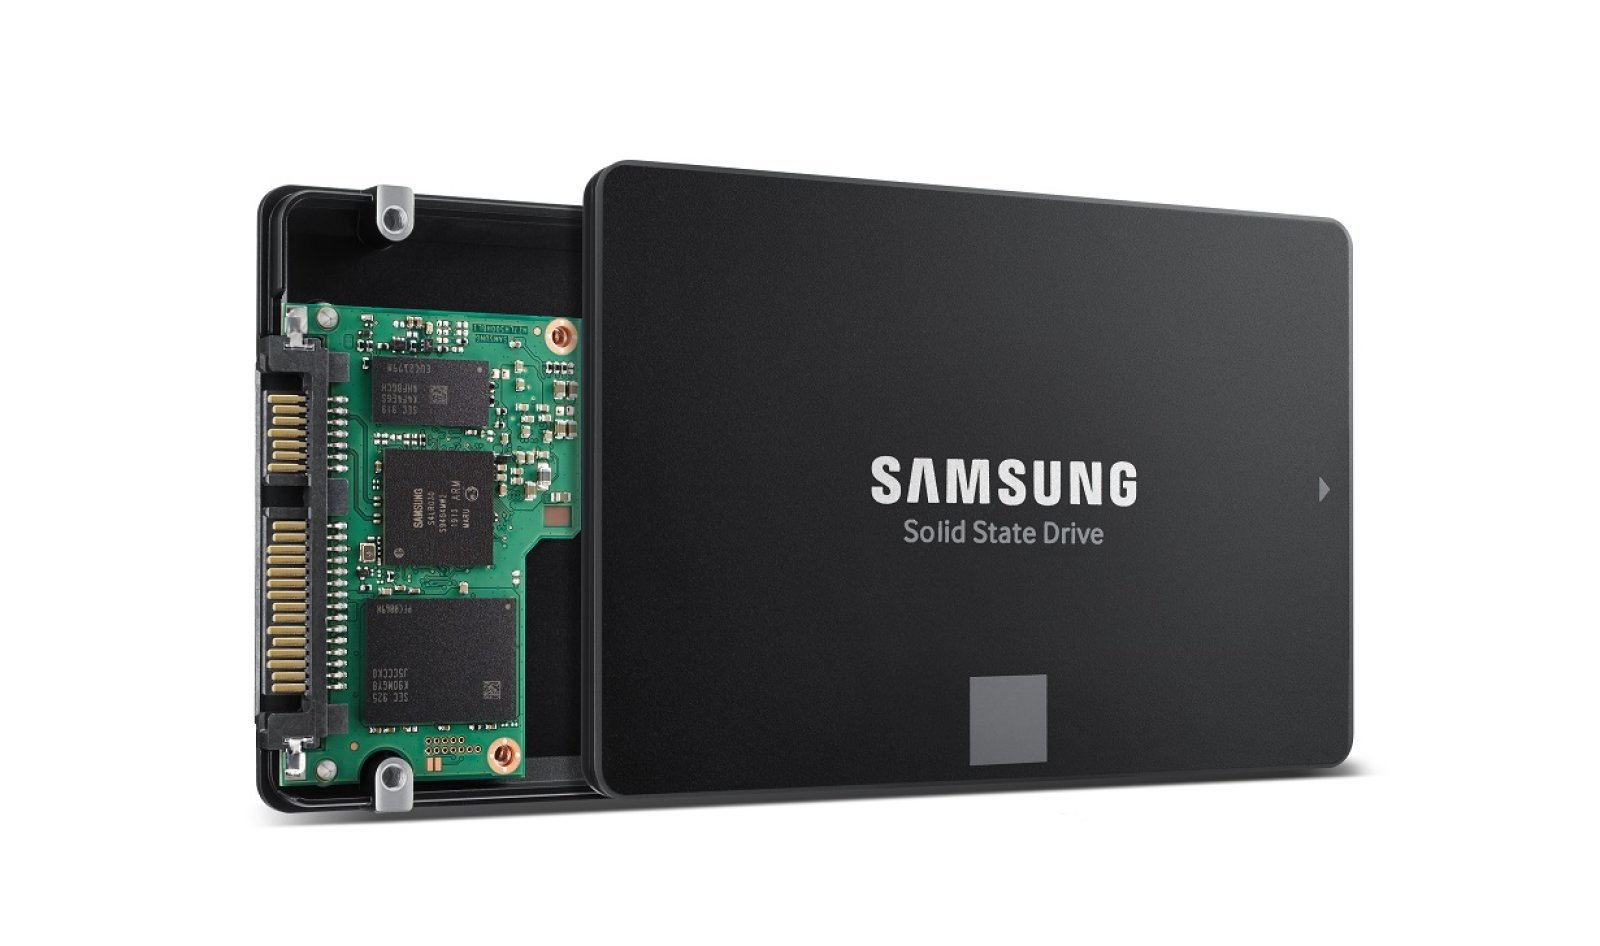
\includegraphics[width=4cm]{SSD.png}
\centering
\caption{Disco de estado solido SSD}
\label{fig:Disco de estado solido SSD}
\end{figure}

Simplemente son un cuarto de archivos más rápido, entre 7 y 10 veces más rápido, y mejora muchísimo los tiempos de lectura y de escritura, teniendo en cuenta que lo más lento que hace tu PC es cargar y escribir de disco, se nota muchísimo la diferencia.\\


El SSD también almacena los datos en celdas, muy parecido a cómo funciona una RAM, El problema que tienen este tipo de celdas, es que son como pequeñas baterías, con el tiempo se van deteriorando y cada vez pierden un poco más su capacidad para almacenar datos con un cierto número de ciclos de lectura y escritura acabaría siendo inutilizable, por eso los SSD no son tan fiables como un disco duro tradicional, pero claro, todo depende del uso que se le vaya a dar.\\

Si escribes y borrás datos continuamente pues menos tiempo te durará tu unidad de estado sólido.\\

\subsection{VRAM}

\begin{figure}[h]
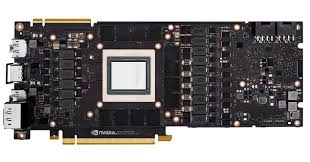
\includegraphics[width=4cm]{VRAM.PNG}
\centering
\caption{Memoria VRAM}
\label{fig:Memoria VRAM}
\end{figure}

Es la memoria de tu tarjeta gráfica, este tipo de RAM funciona de forma muy similar a la RAM de tu computador, digamos que la diferencia es que la VRAM es capaz de descargar muchos más datos de golpe, pero sin embargo cada vez que vas a buscar los datos tarda bastante más.\\

El proceso de pedir datos es más lento, pero sin embargo los datos que te llegan vienen en mayor cantidad, esto es mucho mejor para la tarjeta gráfica porque mientras tú eres el procesador y vas cambiando de informe a menudo ya que sólo puedes trabajar con uno a la vez, vas a hacer un montón de peticiones una tras otra a tu estantería y vas a cambiar de informe constantemente, Sin embargo, la tarjeta gráfica trabaja como si fueran un montón de secretarios trabajando en un montón de informes a la vez.\\ 

Cada vez que vas a buscar informes a la estantería, te conviene tener la capacidad de traer muchísimos a la vez para que los secretarios puedan trabajar con ellos, por eso para la gráfica es mucho mejor recibir más datos de golpe y por eso la RAM de gráfica no es la misma que la memoria principal.\\ 

En fín, como conclusión unas son lentas pero fiables, otras rápidas pero volátiles, otras rapidísimas pero voluminosas, mientras que otras pueden proveer más datos a la vez pero demoran más por cada lectura, cada memoria tiene sus pros y sus contras. Por ese motivo un computador utiliza tantas.\\

Esto nos obliga a estar moviendo de arriba abajo constantemente los datos para evitar crear cuellos de botella o por lo menos minimizarlos si los procesadores no fueran tan rápidos probablemente con la RAM tendríamos suficiente pero hemos llegado a puntos en los cuales si realmente no tenemos todos estos niveles, el procesador se quedaría esperando la mayoría del tiempo es un sistema de memorias para dar la máxima eficiencia a nuestros procesadores, quizás algún día consigamos desarrollar un tipo de memoria muy rápido, muy fiable y muy compacto que sea capaz  de sustituir a la mayoría de estas memorias.\\



\subsection{Memoria Caché}

Estos módulos de memoria están dentro del procesador, existen varios niveles tres o incluso cuatro
podríamos considerar como que tu mesa es el nivel 1 mientras que los distintos cajones del escritorio son los siguientes niveles.


\subsection{Memoria ROM}
Este tipo de memoria es permanente, una vez que se carga información en ellas no se pueden modificar, estas son memorias no volátiles porque, aunque se corte el suministro de corriente eléctrica su información no se ve afectada, normalmente estas memorias se les carga la información desde su fabricación.

\subsection{Memoria PROM}
Funciona exactamente igual que la ROM, la diferencia es que esta viene en blanco, el usuario una vez que le carga la información, no podrá modificarla.

\subsection{Memoria EPROM}
Esta memoria tiene como característica principal que la podemos borrar y cargar con información cuantas veces queramos, para realizar el borrado debe usarse luz UV por una pequeña ventana que trae el chip, para evitar el borrado de esta información se debe tapar esta ventana para que los datos se conserven.

\subsection{Memoria EEPROM}
Funciona exactamente igual que la EPROM, pero no necesita de una ventana de cuarzo y luz UV para borrar o grabar información en ella, ya que se puede borrar o grabar datos por medio de pulsos eléctricos.

\subsection{OPTAIN}
Es la nueva tecnología de Intel (3D XPoints Memory), es un tipo de memoria que quizás en el futuro
sustituya al SSD, son bastante rápidas, aunque no tanto como la RAM Actual, sin embargo, estas memorias son muy caras y no existen de grandes capacidades, aún es una tecnología muy reciente.\\

Intel decidió comercializarlas de momento como una capa más, un módulo intermedio entre la RAM y el disco duro otro nivel de memoria que haría que ciertos datos, como por ejemplo digamos los archivos de windows que se cargan cada vez que enciendes el computador o también podría ser tu juego preferido, pudrían estar directamente en este módulo de memoria Optane por lo cual el computador no tardaría nada en arrancar; iría a mirar si los datos están en Optane, y si están ahí los cargaría de esta memoria, en caso que no estuviera, iría directamente al disco duro. \\

En ese tipo de memoria no caben todos los archivos por ese motivo no se usa como disco principal, pero gracias al software de Intel se almacenan los datos más recurrentes para que cada vez que tengas que cargar lo que más sueles usar notes una gran mejora en la velocidad, como este tipo de memoria no es volátil, cuando apagamos el PC no se vacía La RAM, cargaría los datos directamente desde esta memoria haciendo ciertas tareas, las más comunes, aún más rápidamente que con un SSD. \\

Es la tecnología muy prometedora desde luego, pero tendremos que ver cómo evoluciona podríamos decir que es un pequeño cuarto de archivos más cercano, más pequeño y mejor organizado que tu cuarto de archivo habitual.\\

Toda esta red de memorias me hace pensar en las grandes limitaciones que tenemos y en cómo nos las ingeniamos para conseguir computadores cada vez más rápidos por eso muchas veces en la informática, no todos son simples números.\\ 

El número de ciclos no necesariamente significa que tu procesador sea más rápido, el número de cores (Núcleos) tampoco, lo mismo pasa con la memoria RAM, con los discos duros, con las gráficas, prácticamente cualquier componente que tenga tu PC. nunca es simple, todo tiene sus pros, sus contras y sus limitaciones.\\


\section{¿Por qué tantas memorias y como se gestionan en nuestro computador?}
Una de las grandes limitaciones en los computadores es la Memoria. Los PC’s tienen muchas memorias de hecho son demasiadas. \\

Últimamente se habla incluso de una nueva; El módulo Optane de Intel, también es ampliamente conocido que las unidades SSD son muchísimo más rápidas que los discos duros tradicionales. 

\begin{itemize}
    \item ¿por qué?
    \item¿En qué afecta esto a la velocidad? 
    \item¿para qué quieres tantas memorias?
    \item¿No podríamos tener sólo una y utilizar ésta únicamente? 
    \item¿Por qué complicarse tanto la vida?

\end{itemize}

Vamos a manejar el texto que el profesor amablemente nos facilitó para conocer el tema, pero, vamos a ampliarlo un poco más para profundizar el contexto.\cite{youbioit} Supongamos que tú eres el procesador, trabajas en una oficina y tu objetivo es hacer informes. Trabajas en cientos de ellos, incluso varios están relacionados y necesitas constantemente cruzar datos de unos a otros ¡un trabajo de ensueño!\\

La estructura de tu oficina es la siguiente: tienes una mesa llena de papeles una cajonera con más papeles y una estantería detrás tuyo con más papeles, y también Tienes una sala con otros miles y miles de papeles. Lo que estás utilizando en este momento de forma más inmediata lo tienes en el escritorio, pero en el escritorio no te cabe demasiada cosa, para esto tienes la cajonera bastante a mano. Cada cierto tiempo buscas informes en la cajonera, pero claro No todos te caben, para eso utilizas la estantería y lo que no cabe en la estantería irá a un cuarto de archivo.\\

Para un humano sería una completa tortura este trabajo, esto lo realiza el procesador millones de veces por segundo.\\ 

Seguramente hayas oído hablar de que la memoria RAM es muchísimo más rápida que tu disco duro o SSD y para que el procesador no se quede esperando que los datos carguen desde el disco se utiliza la RAM, que es una memoria intermedia.\\

Imagina que no tuvieras ni mesa ni estantería ni nada y tienes que ir a buscar los informes corriendo de una esquina a otra de la sala de archivos, perderías muchísimo tiempo buscando los archivos y trabajarías más bien poco en tus informes, la memoria RAM resuelve este problema, la estantería que tienes detrás RAM es una memoria que hoy en día es capaz de proveer al procesador con varios gigabytes de datos por segundo. Y aquí nace la pregunta:

\subsection{¿Por qué no utilizamos la RAM como disco duro?}

Sería una buena idea, lamentablemente esta memoria es volátil, en cuanto apagamos el ordenador todos los datos desaparecen, es como ver que en esta estantería que tú tienes y que usas en tu día a día cuando te vas a casa la tienes que vaciar y dejar todo en el gran archivo, el disco duro.\\

Hablemos de esa estantería o de la memoria RAM, la memoria principal cercana al procesador le provee de todos los datos que necesita sin tener que ir al gran archivo, que es muchísimo más lento, el verdadero nombre de la memoria principal del computador es DRAM o (Memoria de Acceso Aleatorio Dinámico), se llama dinámica porque los datos se almacenan en una especie de pilas llamadas capacitores que tienden a perder la carga con el tiempo, como esta carga justamente decae es importante volver a escribir los datos cada cierto tiempo, para evitar que los datos desaparezcan. La DRAM es una memoria rápida pero olvidadiza mientras que el disco duro o los SSD son memorias que persisten aun cuando no tienen corriente que les alimente, esto se conoce como No Volátil, y aquí ya empiezan a ser evidentes nuestras carencias tecnológicas, necesitamos dos tipos de memoria en lugar de uno.\\

Tenemos que mover los datos entre una y otra constantemente porque no tenemos una sola memoria que sea buena para todo, si tuvieramos una sola memoria que no fuera volátil, tuviera las capacidades de una unidad de almacenamiento, y la velocidad de una RAM. Desde luego no necesitaríamos estos dos pasos que no dejan de ser un empalme, un parche para que tu PC no se quede esperando encontrar los archivos., Esta es la tecnología que tenemos, conseguir una memoria que unifique ambas es uno de los retos de la informática hoy en día, y es algo que se está investigando actualmente por varias empresas y universidades, pero no termina aquí.\\

\section{¿Qué tan rápidas son las memorias y por qué esto es importante?}

¿La RAM es rápida? Si, pero no lo suficientemente rápida para que nuestro procesador pueda trabajar a máxima eficiencia, si sólo utilizamos la RAM, el procesador se quedaría en el limbo por ratos esperando que la RAM encuentre los archivos que busca por eso existe otro nivel más de memoria. Resulta que en la evolución de los procesadores llegó un momento en el cual los procesadores eran tan rápidos que la RAM se le quedaba corta de velocidad, el procesador se quedaba cada cierto tiempo esperando que la RAM cargara datos. Así que se introdujo un nuevo nivel de memoria, varios en realidad, resulta que existe un tipo de memoria más rápida que la DRAM.

\subsection{¿Por qué no se usa la SRAM para crear unidades que hagan el trabajo de los discos duros y de la RAM la vez?}

En teoría sería muchísimo más rápido y no necesitaríamos caché, pero resulta que también tiene sus problemas; se habla mucho de que esta memoria es excesivamente cara y si se hiciera un disco duro con este tipo de memoria sería costosísimo. Es verdad que sería algo más caro, pero tampoco es este exactamente el motivo, el problema es que la SRAM requiere 6 transistores por cada celda de memoria mientras que la DRAM sólo 1. O sea que para almacenar un solo bit la SRAM requiere seis veces el número de transistores que la de DRAM efectivamente esto lo hace más caro claro, pero el problema principal es el espacio físico, se necesita mucho más espacio por bit que en la RAM. por lo cual cuando más capacidad queremos tener en este tipo de memoria más grande necesitamos que sea su placa o Main board, esto es un problema porque ese tipo de RAM necesita mucho cableado para interconectar las piezas, y entretanto cableado y que las distancias son mayores dado que la placa necesita ser más grande, la electricidad tardaría demasiado en llegar de un componente a otro haciendo que esta memoria “tan rápida” ya no sea “tan rápida” una de las cosas que se busca siempre en este tipo de circuitos es reducir al máximo las distancias. Los electrones que viajan por el circuito tienen cierta velocidad, cuanto más largo es el circuito más lento será. Obviamente las diferencias no son tan grandes pero sí que son muy significativas cuando hablamos de billones de ciclos por segundo.\\

Las memorias caché se dividen en distintos niveles según su densidad. Una placa más densa puede almacenar más datos en un determinado espacio respecto a otras menos densas. En otras palabras
el chip donde está montada la memoria, en el caso que sea una memoria más densa, puede albergar más bits, mientras que una menos densa, menos bits en el mismo espacio cuanto más rápida es la caché más componentes necesita por cada bit. Por eso las memorias más rápidas ocupan más sitio en la placa.\\ 

Cada nivel de caché es más grande y más denso que el anterior, pero también más lento por esta razón cada memoria tiene sus problemas.\\

Esto sería el equivalente a decir: el caché nivel 1, es la mesa. La mesa tiene una capacidad de papeles limitada, si bien los papeles son muy accesibles en la mesa, si quisiéramos hacer una mesa mucho más grande tendríamos el problema de que nos costaría trabajo llegar de una punta a otra de la mesa, como vemos acabamos antes teniendo una cajonera o una estantería detrás con todos los documentos organizados. Si tuvieramos que poner todos los documentos que tenemos en la estantería en una mesa, necesitaríamos una mesa muy grande y sería muy muy poco eficiente. Esto es exactamente lo que pasa con la caché. Si bien la caché de nivel 1 es muy rápida, si quisiéramos tener una caché de nivel 1 del tamaño de la RAM tendría tanto recorrido que sería lenta.\\ 

\bibliographystyle{IEEEtran}
\bibliography{Bibliografia.bib}

\end{document}
